% !TeX root = thesis.tex

\chapter{Software Engineering}

\label{ch:software-engineering}
\acrfull{ieee} defines the practice of Software Engineering as the ``Application of a systematic, disciplined, quantifiable approach to the development, operation and maintenance of software; that is, the application of engineering to software'' \cite[p.~421]{8016712}. The word ``systematic'' in this definition emphasises the need for a structured process, depicting guidelines and models that describe how we should develop software in the most efficient way possible. Such a process does exist under the name of the \acrfull{sdlc} \cite[p.~420]{8016712}. If a developer prefers not to abide by any model and act as they deem correct without following any guidelines, we employ the term \emph{Cowboy coding} \cite[p.~34]{landry2011iterative}.

% !TeX root = ../thesis.tex

\section{Software Development Life Cycle}\label{sec:se-sdlc}
An implementation of the SDLC consists of two major components. First, the process is broken down into several smaller phases. Depending on the nature of the software, it is possible to omit steps or add more steps. I have compiled a simple yet generic approach from multiple sources \cite{2010govardhan, 7106435}, to which most software projects adhere. This approach consists of five phases.
\begin{enumerate}
	\bolditem{Requirements phase} This is the initial phase of the development process. During this phase, the developer gets acquainted with the project and compiles a list of the desired functionalities \cite{7106435}. Using this information, the developer eventually decides on the required hardware specifications and possible external software which will need to be acquired.
	
	\bolditem{Design phase} After the developer has gained sufficient knowledge about the project requirements, they can use this information to draw an architectural design of the application. This design consists of multiple documents, including user stories and UML-diagrams.
	
	\bolditem{Implementation phase} During this phase, the developer will write code according to the specifications defined in the architectural designs.
	
	\bolditem{Testing phase} This is the most important phase. During this phase, the implementation is tested to identify potential bugs before the application is used by other users.
	
	\bolditem{Operational phase} In the final phase, the project is fully completed and it is integrated in the existing business environment.
\end{enumerate}

\noindent Subsequently, a model is chosen to define how to transition from one phase into another phase. A manifold of models exist \cite{2010govardhan}, each having advantages and disadvantages, but I will consider the basic yet most widely used model, which is the Waterfall model by Benington \cite{united1956symposium}. The initial Waterfall model required every phase to be executed sequentially and in order, cascading. However, this imposes several issues, the most prevalent being the inability to revise design decisions taken in the second phase, when performing the actual implementation in the third phase. To mitigate this, an improved version of the Waterfall model was proposed by Royce \cite{Royce:1987:MDL:41765.41801}. This version allows a phase to transition to a previous phase, as illustrated in \autoref{fig:waterfall-royce}.

\begin{figure}[htbp!]
	\centering
	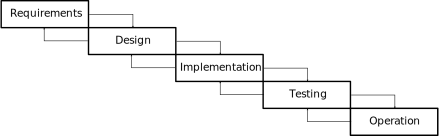
\includegraphics[width=\textwidth]{assets/sdlc.pdf}
	\caption{Improved Waterfall model by Royce}
	\label{fig:waterfall-royce}
\end{figure}

\noindent In this thesis I will solely focus on the implementation and testing phase, as these are the most time-consuming phases of the entire process. The modification to the Waterfall model by Royce is particularly useful when applied to these two phases, in the context of \emph{software regressions}. A regression \cite{10.1007/978-3-540-77966-7_18} is a feature that was previously working correctly, but is now malfunctioning. This behaviour can have external causes, such as a change in the system clock because of daylight saving time, but can also be the result of a change to another, seemingly unrelated part of the application code \cite{6588537}.\\

\noindent Software regressions and other functional bugs can ultimately incur disastrous effects, such as severe financial loss or damage to the reputation of the software company. The most famous example in history is without any doubt the explosion of the Ariane 5-rocket, which was caused by an integer overflow \cite{581900}. In order to reduce the risk of bugs, malfunctioning components should be detected as soon as possible to proactively defend against potential failures. Because of this reason, the testing phase is to be considered as the most important phase of the entire development process and an application should therefore include sufficient tests. The collection of all tests included in an application, or a smaller chosen subset of certain tests, is referred to as the \emph{test suite}. Tests can be classified in multiple categories, this thesis will consider three distinguishable categories:

\begin{enumerate}
	\bolditem{Unit test} This is the most basic kind of test. The purpose of a unit test is to verify the behaviour of an individual component \cite{whittaker2000}. The scope of a unit test should be limited to a small and isolated piece of code, such as one function. Unit tests are typically implemented as \emph{white-box tests} \cite[p.~12]{6588537}. A white-box test is constructed by manually inspecting the function under test, to identify important \emph{edge values}. The unit test should then feed these values as arguments to the function under test, to observe its behaviour. Common edge cases include zero, negative numbers, empty arrays or array boundaries that might result in an overflow.
	
	\bolditem{Integration test} A more advanced test, an integration test verifies the interaction between multiple individually tested components \cite{whittaker2000}. Examples of integration tests include the communication between the front-end and the back-end side of an application. As opposed to unit tests, an integration test is an example of a \emph{black-box} test \cite[p.~6]{6588537}, meaning that implementation-specific details should be irrelevant or unknown when writing an integration test.
	
	\bolditem{Regression test} After a regression has been detected, a regression test \cite[p.~372]{8016712} is added to the test suite. This regression test should replicate the exact conditions and sequence of actions that have caused the regression, to warden the implementation against subsequent failures if the same conditions would reapply in the future.
\end{enumerate}

% !TeX root = ../../thesis.tex

\subsection{Test Suite Assessment}

\subsubsection{Coverage}
\noindent The most frequently used metric to measure the quantity and thoroughness of a test suite is the \emph{code coverage} or \emph{test coverage} \cite[p.~467]{8016712}. The test coverage is expressed as a percentage and indicates which fraction of the application code is affected by code in the test suite. Internally, this works by augmenting every statement in the application code using binary instrumentation. A hook is inserted before and after every statement to keep track of which statements are executed during tests. Many different criteria exist to interpret these instrumentation results and thus to express the fraction of covered code \cite{Myers:2011:AST:2161638}, the most commonly used ones are \emph{statement coverage} and \emph{branch coverage}.

\paragraph*{Statement coverage} expresses the fraction of code statements that are executed in any test of the test suite \cite{6588537}, out of all executable statements in the application code. Analogously, the fraction of lines covered by a test may be used to calculate the \emph{line coverage} percentage. Since one statement can span multiple lines and one line may also contain more than one statement, both of these criteria implicitly represent the same value. Statement coverage is heavily criticised in literature \cite[p.~37]{Myers:2011:AST:2161638}, since it is possible to achieve a statement coverage percentage of 100\% on a code fragment which can be proven to be incorrect. Consider the code fragment in \autoref{lst:statement-coverage-fail}. If a test would call the \texttt{example}-function with arguments $\{a = 1, b = 2\}$, the test will pass and every statement will be covered, resulting in a statement coverage of 100\%. However, it is clear to see that if the function would be called with arguments $\{a = 0, b = 0\}$, a \emph{division-by-zero} error would be raised, resulting in a crash. This very short example already indicates that statement coverage is not trustworthy, yet it may still be useful for other purposes, such as detecting unreachable code which may safely be removed.

\begin{listing}
	\begin{lstlisting}[language=C]
		int example(int a, int b) {
			if (a == 0 || b != 0) {
				return a / b;
			}
		}
	\end{lstlisting}
	\captionsetup{skip=-2pt}
	\caption{Example of irrelevant statement coverage in C.}
	\label{lst:statement-coverage-fail}
\end{listing}

\paragraph*{Branch coverage} on the other hand, requires that every branch of a conditional statement is traversed at least once \cite[p.~37]{Myers:2011:AST:2161638}. For an \texttt{if}-statement, this results in two tests being required, one for every possible outcome of the condition (\texttt{true} or \texttt{false}). For a \texttt{loop}-statement, this requires a test case in which the loop body is never executed and another test case in which the loop body is always executed. Remark that while this criterion is stronger than statement coverage, it is still not sufficiently strong to detect the bug in \autoref{lst:statement-coverage-fail}. In order to mitigate this, \emph{multiple-condition coverage} \cite[p.~40]{Myers:2011:AST:2161638} is used. This criterion requires that for every conditional statement, every possible combination of subexpressions is evaluated at least once. Applied to \autoref{lst:statement-coverage-fail}, the \texttt{if}-statement is only covered if the following four cases are tested, which is sufficient to detect the bug.
\begin{itemize}
	\item $a = 0, b = 0$
	\item $a = 0, b \neq 0$
	\item $a \neq 0, b = 0$
	\item $a \neq 0, b \neq 0$
\end{itemize}

\noindent It should be self-evident that achieving and maintaining a coverage percentage of 100\% at all times is critical. However, this does not necessarily imply that all lines, statements or branches need to be covered explicitly \cite{dein_2019}. Some parts of the code might simply be irrelevant or untestable. Examples include wrapper or delegation methods that simply call a library function. All major programming languages have frameworks and libraries available to collect coverage information during test execution, and each of these frameworks allows the developer to exclude parts of the code from the final coverage calculation. As of today, the most popular options are JaCoCo\footnote{\url{https://www.jacoco.org/jacoco/}} for Java, coverage.py\footnote{\url{https://github.com/nedbat/coveragepy}} for Python and simplecov\footnote{\url{https://github.com/colszowka/simplecov}} for Ruby. These frameworks are able to generate in-depth statistics on which parts of the code are covered and which parts require more tests, as illustrated in \autoref{fig:coverage-statistics}.

\subsubsection{Mutation testing}
Whereas code coverage can be used to identify whether or not a part of the code is currently affected by the test suite, \emph{mutation testing} can be used to measure its quality and ability to detect future failures. This technique creates several syntactically different instances of the source code, referred to as \emph{mutants}. A mutant can be created by applying one or more \emph{mutation operators} to the original source code. These mutation operators are aimed at simulating typical mistakes that developers tend to make, such as the introduction of off-by-one errors, removal of statements and replacement of logical connectors \cite{Offutt2001}. The \emph{mutation order} refers to the amount of mutation operators that have been applied consecutively to an instance of the code. This order is traditionally rather low, as a result of the \emph{Competent Programmer Hypothesis}, which states that programmers develop programs which are near-correct \cite{5487526}.

\paragraph*{Creating and evaluating} the mutant versions of the code is a computationally expensive process and requires human intervention, which is why very few software developers have managed to employ this technique in practice. \autoref{fig:mutation-testing} shows how mutation testing is performed. First of all, the mutation system takes the original program $P$ and a set of test cases $T$. Then, several mutation operators are applied to construct a large set of mutants $P'$. The next step is to evaluate every test case $t$ on the original program $P$ to verify its correctness, this is a task that needs to be performed manually. If at least one of these test cases proves incorrect, a bug has been found in the original program, which needs to be resolved before the mutation analysis can continue. When $P$ successfully passes every test case, every test case are evaluated for each of the mutants. A mutant $p'$ is said to be ``killed'' if its output is different from $P$ for at least one test case, otherwise it is considered ``surviving''. After executing all test cases, the set of surviving mutants should be analysed in order to introduce subsequent test cases that can be used to kill them. However, it is also possible that the surviving mutants are functionally equivalent to $P$. This needs to be verified manually, since the detection of program equivalence is impossible \cite{5487526, Offutt2001}.

\begin{figure}[htbp!]
	\centering
	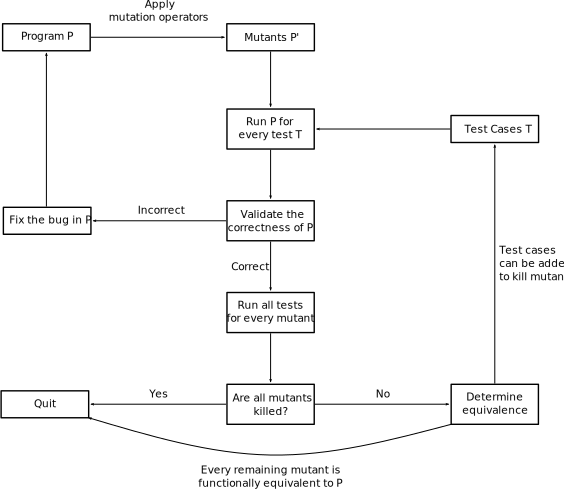
\includegraphics[width=\textwidth]{assets/mutation-testing.pdf}
	\caption{Process of Mutation Testing (based on \cite{Offutt2001})}
	\label{fig:mutation-testing}
\end{figure}

\noindent After every mutant has either been killed or marked equivalent to the original problem, a \emph{mutation score} is calculated using \autoref{eq:mutant-score}. In a perfect test suite, this score should be equal to 1, indicating that the test suite was able to detect every mutant. 

\begin{equation}\label{eq:mutant-score}
	\text{Mutant Score} = \frac{\text{killed mutants}}{\text{non-equivalent mutants}}
\end{equation}


\begin{figure}[htbp!]
	\centering
	\subfloat[JaCoCo coverage report of \url{https://github.com/thepieterdc/dodona-api-java}]{%
		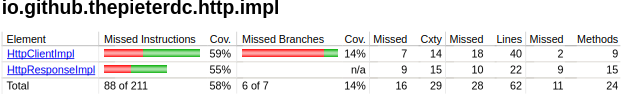
\includegraphics[clip,width=\textwidth]{assets/coverage-jacoco.pdf}
	}
	\newline
	\subfloat[coverage.py report of \url{https://github.com/codecov/example-python}]{%
		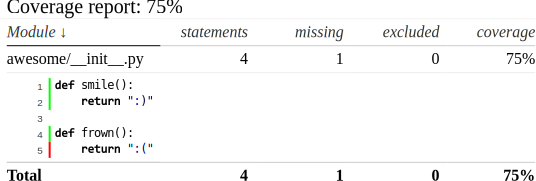
\includegraphics[clip,width=\textwidth]{assets/coverage-coveragepy.pdf}
	}
	\newline
	\subfloat[simplecov report of \url{https://github.com/dodona-edu/dodona}]{%
		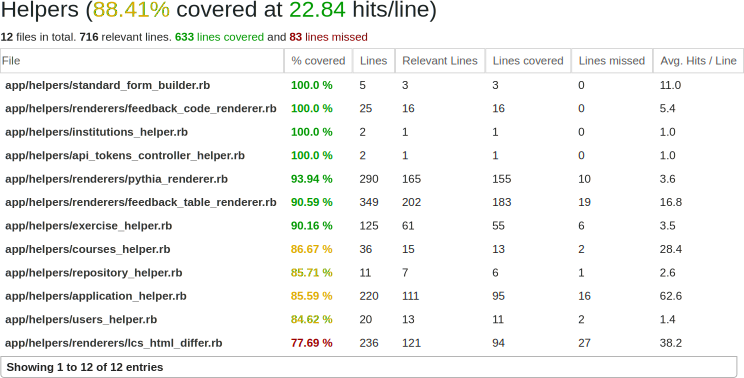
\includegraphics[clip,width=\textwidth]{assets/coverage-simplecov.pdf}
	}
	\caption{Statistics from Code coverage tools}
	\label{fig:coverage-statistics}
\end{figure}
% !TeX root = ../../thesis.tex

\subsection{Test Suite Assessment}

\subsubsection{Coverage}
\noindent The most frequently used metric to measure the quantity and thoroughness of a test suite is the \emph{code coverage} or \emph{test coverage} \cite[p.~467]{8016712}. The test coverage is expressed as a percentage and indicates which fraction of the application code is affected by code in the test suite. Internally, this works by augmenting every statement in the application code using binary instrumentation. A hook is inserted before and after every statement to keep track of which statements are executed during tests. Many different criteria exist to interpret these instrumentation results and thus to express the fraction of covered code \cite{Myers:2011:AST:2161638}, the most commonly used ones are \emph{statement coverage} and \emph{branch coverage}.

\paragraph*{Statement coverage} expresses the fraction of code statements that are executed in any test of the test suite \cite{6588537}, out of all executable statements in the application code. Analogously, the fraction of lines covered by a test may be used to calculate the \emph{line coverage} percentage. Since one statement can span multiple lines and one line may also contain more than one statement, both of these criteria implicitly represent the same value. Statement coverage is heavily criticised in literature \cite[p.~37]{Myers:2011:AST:2161638}, since it is possible to achieve a statement coverage percentage of 100\% on a code fragment which can be proven to be incorrect. Consider the code fragment in \autoref{lst:statement-coverage-fail}. If a test would call the \texttt{example}-function with arguments $\{a = 1, b = 2\}$, the test will pass and every statement will be covered, resulting in a statement coverage of 100\%. However, it is clear to see that if the function would be called with arguments $\{a = 0, b = 0\}$, a \emph{division-by-zero} error would be raised, resulting in a crash. This very short example already indicates that statement coverage is not trustworthy, yet it may still be useful for other purposes, such as detecting unreachable code which may safely be removed.

\begin{listing}
	\begin{lstlisting}[language=C]
		int example(int a, int b) {
			if (a == 0 || b != 0) {
				return a / b;
			}
		}
	\end{lstlisting}
	\captionsetup{skip=-2pt}
	\caption{Example of irrelevant statement coverage in C.}
	\label{lst:statement-coverage-fail}
\end{listing}

\paragraph*{Branch coverage} on the other hand, requires that every branch of a conditional statement is traversed at least once \cite[p.~37]{Myers:2011:AST:2161638}. For an \texttt{if}-statement, this results in two tests being required, one for every possible outcome of the condition (\texttt{true} or \texttt{false}). For a \texttt{loop}-statement, this requires a test case in which the loop body is never executed and another test case in which the loop body is always executed. Remark that while this criterion is stronger than statement coverage, it is still not sufficiently strong to detect the bug in \autoref{lst:statement-coverage-fail}. In order to mitigate this, \emph{multiple-condition coverage} \cite[p.~40]{Myers:2011:AST:2161638} is used. This criterion requires that for every conditional statement, every possible combination of subexpressions is evaluated at least once. Applied to \autoref{lst:statement-coverage-fail}, the \texttt{if}-statement is only covered if the following four cases are tested, which is sufficient to detect the bug.
\begin{itemize}
	\item $a = 0, b = 0$
	\item $a = 0, b \neq 0$
	\item $a \neq 0, b = 0$
	\item $a \neq 0, b \neq 0$
\end{itemize}

\noindent It should be self-evident that achieving and maintaining a coverage percentage of 100\% at all times is critical. However, this does not necessarily imply that all lines, statements or branches need to be covered explicitly \cite{dein_2019}. Some parts of the code might simply be irrelevant or untestable. Examples include wrapper or delegation methods that simply call a library function. All major programming languages have frameworks and libraries available to collect coverage information during test execution, and each of these frameworks allows the developer to exclude parts of the code from the final coverage calculation. As of today, the most popular options are JaCoCo\footnote{\url{https://www.jacoco.org/jacoco/}} for Java, coverage.py\footnote{\url{https://github.com/nedbat/coveragepy}} for Python and simplecov\footnote{\url{https://github.com/colszowka/simplecov}} for Ruby. These frameworks are able to generate in-depth statistics on which parts of the code are covered and which parts require more tests, as illustrated in \autoref{fig:coverage-statistics}.

\subsubsection{Mutation testing}
Whereas code coverage can be used to identify whether or not a part of the code is currently affected by the test suite, \emph{mutation testing} can be used to measure its quality and ability to detect future failures. This technique creates several syntactically different instances of the source code, referred to as \emph{mutants}. A mutant can be created by applying one or more \emph{mutation operators} to the original source code. These mutation operators are aimed at simulating typical mistakes that developers tend to make, such as the introduction of off-by-one errors, removal of statements and replacement of logical connectors \cite{Offutt2001}. The \emph{mutation order} refers to the amount of mutation operators that have been applied consecutively to an instance of the code. This order is traditionally rather low, as a result of the \emph{Competent Programmer Hypothesis}, which states that programmers develop programs which are near-correct \cite{5487526}.

\paragraph*{Creating and evaluating} the mutant versions of the code is a computationally expensive process and requires human intervention, which is why very few software developers have managed to employ this technique in practice. \autoref{fig:mutation-testing} shows how mutation testing is performed. First of all, the mutation system takes the original program $P$ and a set of test cases $T$. Then, several mutation operators are applied to construct a large set of mutants $P'$. The next step is to evaluate every test case $t$ on the original program $P$ to verify its correctness, this is a task that needs to be performed manually. If at least one of these test cases proves incorrect, a bug has been found in the original program, which needs to be resolved before the mutation analysis can continue. When $P$ successfully passes every test case, every test case are evaluated for each of the mutants. A mutant $p'$ is said to be ``killed'' if its output is different from $P$ for at least one test case, otherwise it is considered ``surviving''. After executing all test cases, the set of surviving mutants should be analysed in order to introduce subsequent test cases that can be used to kill them. However, it is also possible that the surviving mutants are functionally equivalent to $P$. This needs to be verified manually, since the detection of program equivalence is impossible \cite{5487526, Offutt2001}.

\begin{figure}[htbp!]
	\centering
	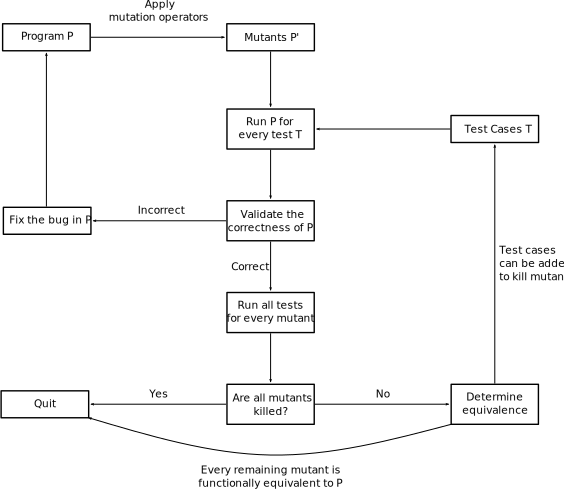
\includegraphics[width=\textwidth]{assets/mutation-testing.pdf}
	\caption{Process of Mutation Testing (based on \cite{Offutt2001})}
	\label{fig:mutation-testing}
\end{figure}

\noindent After every mutant has either been killed or marked equivalent to the original problem, a \emph{mutation score} is calculated using \autoref{eq:mutant-score}. In a perfect test suite, this score should be equal to 1, indicating that the test suite was able to detect every mutant. 

\begin{equation}\label{eq:mutant-score}
	\text{Mutant Score} = \frac{\text{killed mutants}}{\text{non-equivalent mutants}}
\end{equation}


\begin{figure}[htbp!]
	\centering
	\subfloat[JaCoCo coverage report of \url{https://github.com/thepieterdc/dodona-api-java}]{%
		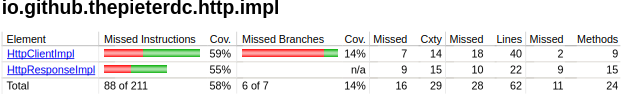
\includegraphics[clip,width=\textwidth]{assets/coverage-jacoco.pdf}
	}
	\newline
	\subfloat[coverage.py report of \url{https://github.com/codecov/example-python}]{%
		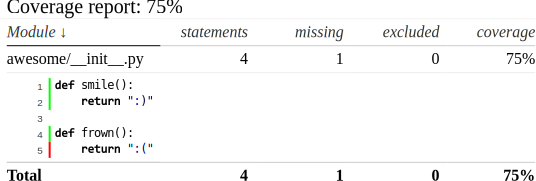
\includegraphics[clip,width=\textwidth]{assets/coverage-coveragepy.pdf}
	}
	\newline
	\subfloat[simplecov report of \url{https://github.com/dodona-edu/dodona}]{%
		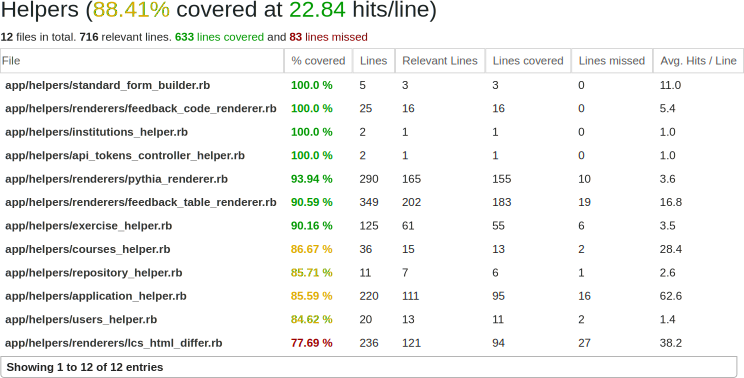
\includegraphics[clip,width=\textwidth]{assets/coverage-simplecov.pdf}
	}
	\caption{Statistics from Code coverage tools}
	\label{fig:coverage-statistics}
\end{figure}
\newpage
% !TeX root = ../thesis.tex

\section{Agile Software Development}
% !TeX root = ../../thesis.tex

\subsection{Agile Manifesto}
Since the late 1990s, developers have tried to reduce the time occupied by the implementation and testing phases. As a result, several software pioneers have proposed new implementations of the SDLC, which were later collectively referred to as the \emph{Agile development methodologies}. This term was coined during a meeting of seventeen prominent software developers, in which they have defined the following four fundamental values of Agile development in the \emph{Agile Manifesto} \cite{beck2001agile}.

\begin{enumerate}
	\item \emph{Individuals and interactions} over processes and tools.
	\item \emph{Working software} over comprehensive documentation.
	\item \emph{Customer collaboration} over contract negotiation.
	\item \emph{Responding to change} over following a plan.
\end{enumerate}

\noindent According to the authors, we should interpret these values as follows: ``While there is value in the items on the right, we value the items on the left more'' \cite{beck2001agile}. When we examine these values more closely, we can observe that they all share a common philosophy, which is that software engineering should be a fast process in which communication and a short feedback loop is critical to avoid missteps. Since 2001, a variety of different programming models have arisen, each incorporating these Agile principles in their own way. The most remarkable new practice is \acrfull{tdd}. Recall that an integration test is a black-box test and that as such, we can actually construct the test case in advance and write the implementation afterwards. This concept is also prevalent in TDD. This practice depicts that if we want to extend the functionality of the application, we should first modify the test cases (or add new test cases) and then modify the application code until every test case is passing \cite{10.5555/579193}.
% !TeX root = ../../thesis.tex

\subsection{The need for Agile}
In the wake of the world economic crisis, software companies were forced to devote efforts into researching how their overall expenses could be reduced. This research has concluded that in order to reduce financial risks, the \emph{time-to-market} of an application should be as short as possible. In order to accomplish this, further research was conducted, resulting in an increase of attention for agile methodologies in scientific literature \cite{ionel2009}. As was previously described in \autoref{sssec:agilevalue-workingsoftware}, agile methodologies strive to deliver a minimal version as soon as possible, allowing additional functionality to be added in an incremental fashion. This effectively results in a shorter \emph{time-to-market} and lower costs, since the company can decide to cancel the project much earlier in the process.\\

\noindent In addition to a reduced time-to-market, maintaining an agile workflow has also proven beneficial to the success rate of development. A study performed by The Standish Group revealed that the success rate of agile projects is more than three times higher compared to when traditional methodologies are practised \cite[p.~7]{standish2015chaos}, as illustrated in \autoref{fig:agile-success-rate}. 

\begin{figure}[htbp!]
	\centering
	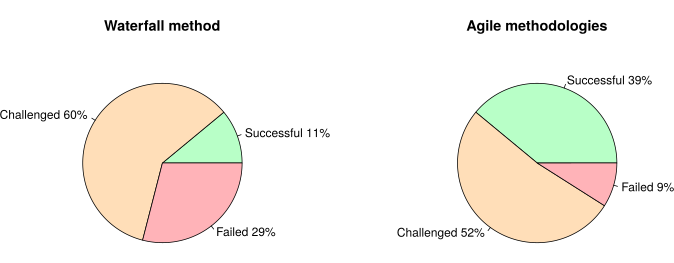
\includegraphics[width=\textwidth]{assets/agile-success-rate.pdf}
	\caption{Success rate of Agile methodologies \cite{standish2015chaos}.}
	\label{fig:agile-success-rate}
\end{figure}



%hier in hoofdstuk 7 staat iets over continuous integration
%https://link.springer.com/chapter/10.1007/978-3-319-05155-0_7

- changes moeten zeer regelmatig worden geintegreerd met elkaar -> feedback loop tussen implement -> integrate -> test -> repeat
- Continuous integration: wat?
- Bestaan aantal bestaande frameworks voor
- Maar; dat testen kan heel lang duren (zoek een bron waarin lange tests besproken worden)
- Bestaan aantal oplossingen voor -> zie volgende hoofdstuk

- feedback loop

- buildup naar waarom tooling nodig is

- waarom

- wat

- voorbeelden: Jenkins, CircleCI, Travis-CI, recent GitHub Actions + screenshots

- Probleem en oplossingen met regression tests


\section{Continuous Integration}
\subsection{Agile Manifesto}
Since the late 1990's, developers have tried to reduce the time occupied by the implementation and testing phases. In order to accomplish this, several new implementations of the SDLC were proposed and evaluated, later collectively referred to as \emph{Agile development methodologies}. The term \emph{Agile development} was coined during a meeting of seventeen prominent software developers, held between February 11-13, 2001, in Snowbird, Utah \cite{jimhighsmith2001}. As a result of this meeting, the developers defined the four key values and twelve principles that define these new methodologies, called the \emph{Manifesto for Agile Software Development}, also known as the \emph{Agile Manifesto}.

\subsubsection{Four values}

The four key values of Agile programming should be interpreted as follows, according to the authors: "While there is value in the items on the right, we value the items on the left more" \cite{beck2001agile}. It should be noted that these values are merely guidelines and that no concrete implementation is provided. A variety of different programming models have arisen since 2001, each incorporating these values in their own unique way.

// TODO ZIE hazzan2014 paper

\begin{enumerate}
	\item \textbf{\emph{Individuals and interactions} over processes and tools:} (TODO explain)
	\item \textbf{\emph{Working software} over comprehensive documentation:} (TODO explain)
	\item \textbf{\emph{Customer collaboration} over contract negotiation:} (TODO explain)
	\item \textbf{\emph{Responding to change} over following a plan:} (TODO explain)
\end{enumerate}

\subsubsection{Twelve principles}
\begin{enumerate}
	\item \textbf{(TODO principle 1)} (TODO explain)
	\item \textbf{(TODO principle 2)} (TODO explain)
	\item \textbf{(TODO principle 3)} (TODO explain)
	\item \textbf{(TODO principle 4)} (TODO explain)
	\item \textbf{(TODO principle 5)} (TODO explain)
	\item \textbf{(TODO principle 6)} (TODO explain)
	\item \textbf{(TODO principle 7)} (TODO explain)
	\item \textbf{(TODO principle 8)} (TODO explain)
	\item \textbf{(TODO principle 9)} (TODO explain)
	\item \textbf{(TODO principle 10)} (TODO explain)
	\item \textbf{(TODO principle 11)} (TODO explain)
	\item \textbf{(TODO principle 12)} (TODO explain)
\end{enumerate}

\subsection{The need for Agile}
Over the past decade, the agile methodologies have received increasing attention amongst software developers, following the world economic crisis of 2009 \cite{ionel2009}. A consequence of this crisis was that software companies were forced to cut on their expenses and find ways to reduce the \emph{time-to-market} of their applications.

- probleem met waterfall model -> een bron hiervoor?

- feedback loop

- buildup naar waarom tooling nodig is

- waarom

- wat

- voorbeelden: Jenkins, CircleCI, Travis-CI, recent GitHub Actions + screenshots

- Probleem en oplossingen met regression tests

  - Test Case Prioritization -> Focus want geen tests weggooien
  
  - Test Suite Minimization
  
  - Test Suite Selection
  
  - Test Suite Reduction

